% FEUP THESIS STYLE for LaTeX2e
% how to use feupteses (changed from the original for MIEEC)
%
% FEUP, JCL & JCF, Tue May 20 18:53:15 2008
%
% PLEASE send improvements to jlopes at fe.up.pt, jcf at fe.up.pt
%

%%========================================
%% Commands: pdflatex mieic
%%           bibtex mieic
%%           makeindex mieic (only if crating an index) 
%%           pdflatex mieic
%%========================================

\documentclass[11pt,a4paper]{report}
%\documentclass[11pt,a4paper]{report}

%% For iso-8859-1 (latin1), comment next line and uncomment the second line
\usepackage[utf8]{inputenc}
\usepackage{amsmath}
\usepackage{amsfonts}
\usepackage{tkz-graph}
\usepackage{tikz-er2}
\usetikzlibrary{calc,arrows,shapes}
%\usepackage[latin1]{inputenc}

%% Use option portuges if needed
\usepackage[english]{babel}

%% For the final version, comment next line and uncomment the second line
\usepackage[provisional,alpharefs]{feupteses}      
%\usepackage[alpharefs]{feupteses} 

%% Options: 
%% - portuges: titles, etc in portuguese
%% - provisional: the thesis has not been approved yet
%% - alpharefs: bibliography references are alphabetic
%% - numericrefs: bibliography references are numbered (in order of citation)
%% ( by default: author-date format of the ``natbib'' package is used 
%%   the portuguese version requires the file ``plainnat-pt.bst'' to be 
%%   present in the same directory )

%% Include MIEIC definitions different from standard style
\usepackage{mieicpatch}

%% Provide a version number in order to keep track of
%% thesis versions (it will printed in the footer of most pages)
%% 

\version{1.0}

%% Uncomment in the final version in order to make version footer disappear
\noversiontrue                 

%% Uncomment to create an index (at the end of the document)
%\makeindex                      

%% Path to the figures directory
%% TIP: use folder ``figures'' to keep all your figures
\graphicspath{{figures/}}       

%%----------------------------------------
%% TIP: if you want to define more macros, use an external file to
%% keep them
%some macro definitions

% format
\newcommand{\class}[1]{{\normalfont\slshape #1\/}}

% entities
\newcommand{\Feup}{Faculdade de Engenharia da Universidade do Porto}
\newcommand{\osm}{OpenStreetMap.org}
\newcommand{\fhp}{Fraunhofer Portugal AICOS}

% Gantt
\newcommand\ganttline[4]{% line, tag, start end
\node at (0,#1) [anchor=base east] {#2};
\fill[gray] (#3/15,#1-.2) rectangle (#4/15,#1+.2);
\draw[black,thick] (#3/15,#1-.2) rectangle (#4/15,#1+.2);}

% Database 
\newcommand\drawdatabase[4]{% label, x, y, text
\begin{scope}
  \draw[color=black, draw=black, very thick] (#2, #3+0.875cm) ellipse (1cm and 0.3cm);
  \draw[color=black, draw=black, very thick] (#2-1cm, #3+0.875cm) -- (#2-1cm, #3-0.375cm);
  \draw[color=black, draw=black, very thick] (#2+1cm, #3-0.375cm) -- (#2+1cm, #3+0.875cm);
  \node (#1) at (#2,#3) {\parbox{2cm}{\begin{center}#4\end{center}}};
  \clip (#2-1cm,#3-0.375cm) rectangle (#2+1cm, #3-1cm);
  \draw[color=black, draw=black, very thick] (#2, #3-0.375cm) ellipse (1cm and 0.3cm);
\end{scope}
}

%%----------------------------------------

%%========================================
%% Start of document
%%========================================
\begin{document}

%%----------------------------------------
%% Information about the work
%%----------------------------------------
\title{Optimisation of municipal solid waste collection routes based on the
containers' fill status data}
\author{Hugo Miguel Pereira Peixoto}
\degree{Dissertation\\[2mm]
Master in Informatics and Computing Engineering}
%% Date of submission
\thesisdate{30$^{th}$ January, 2010}

%% Insert copyright text if used
%\copyrightnotice{Name of the Author, 2008}

\supervisor{Supervisor}{Luís Paulo Reis}{(Ph.D)}
%% Uncomment next line if necessary
\supervisor{Second Supervisor}{Ana Cristina Aguiar}{(Ph.D)}

%% Uncomment committee stuff in the final version
\committeetext{Approved in oral examination by the committee:}
\committeemember{Chair}{Name of the President}{(Title)}
\signature
\committeemember{External Examiner}{Name of the Examiner}{(Title)}
\committeemember{Internal Examiner}{Name of the Examiner}{(Title)}
\committeedate{31$^{st}$ July, 2008}

%% Specify cover logo (in folder ``figures'')
\logo{feup-logo.pdf}

%%----------------------------------------
%% Cover page(s)
%%----------------------------------------
\maketitle
%% Uncomment next line in the final version
%\committeepage

%% Preliminary materials
\StartPrelim
\begin{singlespace}
  %
\chapter*{Abstract}

Fraunhofer Portugal Research Center for Assistive Information and Communication
Solutions is currently developing a system to monitor the fill status of waste
containers. The introduction of a waste container fill status monitoring system
in the city of Porto, Portugal, gives rise to several opportunities. For
example, it allows the development of a detailed analysis of the city's waste
generation distribution and the optimization of waste collection routes.

This document describes the architecture design of the information system to
store and retrieve data regarding the containers' status. Furthermore, it
provides a description of several algorithms that can be used to obtain
efficient collection routes. This optimization problem is modeled as the
\textit{Capacitated Vehicle Routing Problem}. To address this problem, two
approaches were analyzed; the first involves solving the associated
\textit{Asymmetric Traveling Salesman Problem} --- in which vehicle capacity
constraints are ignored --- followed by clustering the resulting tour into
feasible routes. This approach is called \textit{route-first-cluster-second}.
The second approach relies on the usage of a construction heuristic by
Clarke and Wright.

Regarding the optimization of the \textit{Asymmetric Traveling Salesman Problem}
solution, this study compares several techniques: two construction heuristics
--- \textit{greedy} and \textit{repetitive nearest neighbor} --- and three
meta-heuristics --- \textit{hill climbing}, \textit{genetic algorithms} and
\textit{MAX-MIN ant system}. Additionally, \textit{MAX-MIN ant system} was
subjected to a parameter sensibility analysis.

Results show that \textit{MAX-MIN ant system} achieves more efficient routes
when the number of ants is higher, although it increases the algorithm's running
time.  When dealing with a scenario in which there is a limited time-frame, it
is recommended that a low number of ants is used. The algorithm was also shown
to be very sensitive to changes in parameter $\beta$, which indicates if an ant
should give more importance to the distance between two vertices or to the
pheromone levels in that arc. This analysis suggests that $\beta$ should be
close to $20$.

When evaluating the performance of the presented techniques applied to the
\textit{Capacitated Vehicle Routing Problem}, \textit{MAX-MIN ant system}
produced, in average, more efficient routes than the other approaches. 


\chapter*{Resumo}

O Centro de Pesquisa para Soluções de Informação e Comunicação Assistiva da
Fraunhofer Portugal está a desenvolver um sistema de monitorização do estado de
enchimento dos contentores de lixo. A introdução deste sistema na cidade do
Porto dá origem a várias oportunidades. Por exemplo, torna-se possível fazer uma
análise detalhada da distribuição da geração do lixo na cidade. Este projecto
permite, também, implementar um sistema de optimização das rotas de recolha do
lixo.

Este documento descreve o desenho da arquitectura do sistema de informação que
permitirá armazenar --- e disponibilizar --- a informação referente ao estado
dos contentores. O documento oferece também uma descrição de vários algoritmos
que podem ser utilizados para obter rotas de recolha eficientes. Este problema
de optimização pode ser modelado como um problema de planeamento de rotas de
veículos com capacidade limitada (CVRP).  Neste estudo, foram analisadas duas
abordagens para a resolução do CVRP.  A primeira começa por resolver o problema
do caixeiro viajante em grafos assimétricos (ATSP) --- ignorando as restrições
de capacidade --- e, subsequentemente, divide o circuito obtido em rotas que
respeitem as restrições de capacidade dos veículos. Esta técnica chama-se
\textit{route-first-cluster-second}. A segunda abordagem para resolver o CVRP
é baseada numa heurística construtiva, por Clarke e Wright.

Relativamente ao problema de optimização do problema do caixeiro viajante em
grafos assimétricos, foram comparadas várias técnicas: duas heurísticas
construtivas --- \textit{gulosa} e \textit{vizinho mais próximo repetitivo} ---
e três meta-heurísticas --- \textit{subir-a-colina}, \textit{algoritmos
genéticos} e um sistema de formigas chamado \textit{MAX-MIN ant system} (MMAS).
Além da comparação dos vários algoritmos entre si, foi também feita uma análise
de sensibilidade aos parâmetros do MMAS.

Os resultados mostram que o MMAS calcula rotas mais eficientes quando o número
de formigas é mais elevado, apesar de levar a um aumento no tempo de execução do algoritmo.
Quando aplicado a um cenário em que o tempo de execução disponível é limitado,
é recomendado que se utilize um número reduzido de formigas. Também foi possível
mostrar que o algoritmo é bastante sensível a variações no parâmetro $\beta$,
que decide se uma formiga deve dar mais importância à distância entre dois
vértices ou à quantidade de feromonas existente nesse arco. Esta análise mostrou
que o parâmetro $\beta$ deve tomar valores perto de $20$.

A análise do desempenho dos vários algoritmos, relativamente ao problema de
planeamento de rotas de veículos de capacidade limitada, mostrou que o sistema
de formigas obtém, em média, rotas mais eficientes. 

 % the abstract
  %\chapter*{Acknowledgements}

I thank both my supervisors, Prof. Luís Paulo Reis and Prof. Ana Cristina Aguiar,
for their guidance and support.
\\
\\
To Júlio Santos, for providing me with an awesome working environment, and for
his excellent cooking abilities.
\\
\\
To Raquel Rios Correira, for forcing me to work and keeping me company --- I learned a lot about radiation from her.
\\
\\
To NIFEUP, for all the random stuff.

\vspace{10mm}
\flushleft{Hugo ``Wiki'' Peixoto}
  % the acknowledgments
  %\cleardoublepage
\thispagestyle{plain}

\vspace*{8cm}

\begin{flushright}
   \textsl{``In computing, elegance is not a dispensable luxury \\
              but a quality that decides between success and failure''} \\
\vspace*{1.5cm}
            Edsger W. Dijkstra
\end{flushright}
    % initial quotation if desired
  \cleardoublepage
  \pdfbookmark[0]{Table of Contents}{contents}
  \tableofcontents
  \cleardoublepage
  \pdfbookmark[0]{List of Figures}{figures}
  \listoffigures
  \cleardoublepage
  %\pdfbookmark[0]{List of Tables}{tables}
  %\listoftables
  %\cleardoublepage
  \pdfbookmark[0]{Abbreviations}{abbrevs}
  \chapter*{Abbreviations}
\chaptermark{ABBREVIATIONS}

\begin{flushleft}
\begin{tabular}{l p{0.8\linewidth}}
1-SCP	& 1-Skip Collection Problem \\
ACVRP	& Asymmetric Capacitated Vehicle Routing Problem \\
ARP	& Arc Routing Problem \\
AVRP	& Asymmetric Vehicle Routing Problem \\
BPP	& Bin Packing Problem \\
CARP	& Capacitated Arc Routing Problem \\
CGRP-m	& see MCGRP \\
CPP	& Chinese Postman Problem \\
GTSP	& Graphical Travelling Salesman Problem \\
GRP	& General Routing Problem \\
MCGRP	& Mixed-graph Capacitated General Routing Problem \\
M-RRVRP	& Multiple Rollon-Rolloff Vehicle Routing Problem \\
MSW	& Municipal Solid Waste \\
RPP	& Rural Postman Problem \\
RRVRP	& Rollon-Rolloff Vehicle Routing Problem \\
SGTSP	& Steiner Graphical Travelling Salesman Problem \\
TSP	& Travelling Salesman Problem \\
VRP	& Vehicle Routing Problem \\
\end{tabular}
\end{flushleft}

  % the list of abbreviations used
\end{singlespace}

%%----------------------------------------
%% Body
%%----------------------------------------
\StartBody

%% TIP: use a separate file for each chapter
\chapter{Introduction} \label{chap:intro}

\section*{}


\section{Context and Motivation}
\label{section:context}

Municipal solid waste (MSW) production has been increasing in the last few
years, along with economic growth\citep{McCarthy94}. This has led to the need
--- and subsequent development --- of efficient waste management solutions.
Waste management involves not only the collection, but also the transportation,
recycling and disposal of generated waste.

One can find several case studies reporting the methodologies used by different
countries, as well as reports describing the MSW generation quantities and
patterns.

According to \citet{Bhat1996}, up to 85\% of some cities' waste management
budget spent goes to MSW collection and disposal. With this in mind, route
optimization can be considered as an important field of study regarding the
improvement of MSW management processes.

Many cities around the world have studied and applied several optimization
techniques to their collection scenarios, which can be very different from each
other. In Portugal, however, there seems to be little research regarding this
subject. \citet{Passaro200397} describes the waste management scenario in
Portugal from 1996 and 2002, a period in which several improvements were made
due to changes in the legislation. In 2006, \citet{Magrinho20061477} further
report the legislation trends and present some statistics on the average MSW
generation rate. Concerning collection routing, \citet{Teixeira04} describes a
study for optimizing the collection of urban recyclable waste in the
centre-littoral region of Portugal.




\section{Fill Status Monitoring}
\label{section:monitoring}

The Municipality of Porto, Portugal, is working together with the Fraunhofer
Portugal Research Center for Assistive Information and Communication Solutions
(FhP-AICOS) in order to implement a platform that allows the real-time
measurement of waste containers' fill status. This requires the deployment of
low cost sensors in each container and the development of a communication
system to gather information. On top of this platform, several applications
will then be possible. As an example, this will allow researchers to study
waste generation behaviours on a more detailed level. These monitoring systems
have been studied in places, such as Pudong New Area, in Shanghai,
China\citep{Rovetta09,Vicentini09} and Sweden\citep{Johansson06}.

Another application for this system is the optimisation of waste collection
routes.




\section{Optimisation of Waste Collection Routes}
\label{section:optimization}

The problem of optimising waste collection routes involves deciding, for
example, which streets must each garbage truck follow, which containers should
each one of them collect and how many trucks should a fleet for a given city
have.

One of the first articles regarding this subject was done in
1974\citep{Beltrami74}, and it was applied to both New York and Washington
D.C., United States of America. Since then, several other cities have tried to
minimise the costs involving waste collection: Trabon,
Turkey\citep{Apaydin2007}; Barcelona, Spain\citep{Bautista2004}; Athens,
Greece\citep{Karadimas2005}; Hanoi, Vietnam\citep{Tung2000}; Porto Alegre,
Brazil\citep{Li2008} and many others. 

However, many of these studies do not have real-time information of the
containers' fill status. Usually, they are either based on statistical data
(surveys), or they ignore the containers' fill status and simply collect the
waste in every container.

Combining these techniques with the \textit{Fill Status Monitoring} platform
described in section~\ref{section:monitoring}, the municipality of Porto,
Portugal might reduce even further the collection costs. The main objective of
this work is to develop a solution for route optimisation based on the
previously presented platform.



\section{Objectives}
\label{section:objectives}

With the deployment of a fill status monitoring solution in the municipality
of Porto, there is the need to develop an optimisation framework for the
waste collection routes.

There are two scenarios that will need optimisation. First, there is a
scenario similar to the \textit{Rollon-Rolloff} scenario. Second, a
\textit{commercial} scenario will also be evaluated. The difference between
these can be seen in Chapter~\ref{chap:sota}.

Other than the optimisation process, there is also the need to develop an
architecture to store and retrieve, when necessary, the information obtained
from the fill sensors.


\section{Organisation}

Chapter~\ref{chap:sota} starts by presenting the optimisation of collection routes.
First, an informal description of each scenario is given. Then, each one of the
scenarios is exposed as a mathematical formulation, followed by possible
techniques that can be applied to them.

Chapter~\ref{chap:approach} introduces the optimisation framework being
developed. Three modules are proposed and detailed, and the progress on each
one is presented.

Chapter~\ref{chap:work} presents a work plan for the project.  The work plan
contains both the specification of the tasks, as well as a calendarisation.

 
\chapter{State of the art}
\label{chap:sota}

\section*{}

This chapter describes several studies regarding the optimization of solid
waste collection routes. It reviews the mathematical models used in these
studies and provides alternative optimization techniques that can be applied to
each one.

In section~\ref{section:problem}, the waste collection problem will be
detailed. Section~\ref{section:over-rp} provides a background on the
categorization of routing problems. As a final introductory section,
section~\ref{section:city-graph} exposes the basic data structure used in waste
collection problems.

Sections~\ref{section:residential}, \ref{section:commercial} and
\ref{section:rrvrp} describe each one of the three possible scenarios. Each
section presents a mathematical formulation of the problem, along with
techniques for solving it.

As seen in section~\ref{section:commercial}, waste collection in a commercial
scenario can be divided into two common subproblems; one of them is modeled as
the \textit{Traveling Salesman Problem} (TSP).


\section{General problem description}
\label{section:problem}

Authors of \citet{Golden01} divided waste collection routing problems into
three main categories. First, the commercial collection contemplates waste
collection from businesses and organizations like malls, factories and such.
Second, the residential collection problem involves collecting household
generated waste, usually stored in containers along the streets of a city.
Comparatively, the number of containers in the commercial problem is
significantly smaller than in the residential case.

In both of these two variants, each waste collection vehicle travels to a
container, loads its contents into its hopper and moves on to the next
container. As soon as the hopper is full, the vehicle travels to a disposal
facility (such as a landfill, or a recycling/treatment facility) and deposits
the collected waste.

The third variant --- named Rollon-Rolloff, which is described in
\citet{Bodin00} --- involves large containers, which must be transported
to the disposal facilities and replaced by empty ones. Their dimensions impose
that each vehicle can only transport a single container (either full or empty)
at a time. 

In the Rollon-Rolloff original description, each waste collection vehicle can
perform four basic operations:

\begin{itemize}
\item \textbf{Insertion trip} --- the vehicle brings an empty container from
the waste disposal facility (WDF) to a new location;

\item \textbf{Removal trip} --- the vehicle picks up a full container from a
location and leaves it at the WDF;

\item \textbf{Round trip} --- the vehicle picks up a container, brings it to a
waste disposal facility (WDF) for emptying and returns it to its original
location;

\item \textbf{Exchange trip} --- the vehicle leaves the WDF with an empty
container, travels to a location with a full one and switches them, bringing it
back to the WDF.
\end{itemize}

Although round and exchange trips could be considered as being composed by
insertion and removal operations, the authors considered them as separate
actions to avoid the need for modeling extra constraints. For example, in
round trips the same container is brought back to its original place, while
minimizing the time that location stays without a container. In exchange
trips, the target location may not have room for two containers, so an
extra restriction would have to be added, forcing vehicles to pick up the full
one before delivering the new, empty container.

In each of these three main variants, extra parameters can vary. For example,
consider a scenario with either a single or multiple waste disposal facilities.
In the multiple facilities case, an extra restriction may be to balance the
waste disposed at each location.


\subsection{City graph}
\label{section:city-graph}

All three variants described in section~\ref{section:problem} have a common
base for their mathematical models --- waste collection vehicles that travel
along the streets of a given city. To model a city, the common approach is to
define a graph in which each street is represented by one or two arcs
(depending if the street is one or both ways), with street intersections being
the vertices. Each arc may have several associated weights, reflecting the
street distance, the time it takes to transverse it, or some other metric. As
such, a city graph is defined as the ordered tuple $G = (V, E \cup A)$, where
$V$ represent the vertices, $E$ the (undirected) edges and $A$ the (directed)
arcs.

This definition alone does not suffice to realistically represent the possible
vehicle routes, as there are extra restrictions which must be considered,
specially regarding traffic signs. For example: at a given intersection, it may
not be possible to take a left turn if you are arriving from a specific street.
U-turns may also be forbidden, in certain intersections. 

These restrictions can be specified by defining a cost for every pair of arcs
that intersect at a given vertex. $t_{ava^\prime}$ is denoted as being the
cost to go from the arc $a$ to arc $a^\prime$ by making a turn at $v$. If the
arcs do not intersect at that vertex, or if the traffic signs forbid such a
turn, set $t_{ava^\prime} = +\infty$. Further details on this approach can
be seen in \citet{Corberan2002887}.

For now, consider the case in which there is a depot facility, located in
vertex $v_0 \in V$, and that all waste collection vehicles start and finish
their routes there. Consider that there are $K$ vehicles available, and that
each of the $K$ routes can be defined as a set of round trips, each starting at
the depot. The number of round trips in each vehicle route may or may not be
limited. Furthermore, consider vehicles being limited to an amount $Q$ of
waste that they can carry at any given time. This can be either measured in
weight or in volume.


\section{Overview of routing problems}
\label{section:over-rp}

Before presenting the mathematical formulations that can be used to model our
three waste collecting scenarios, this section provides a background on routing
problems. This is useful to understand the concepts applied in the following
sections. Routing problems are an important field in optimization, with many
different applications. Its first formulation is usually attributed to Euler's
article on the briges of Königsberg~\citet{Euler1736}.

The usual underlying structure for these problems is a strongly connected mixed
graph. A mixed graph, $G = (V, E \cup A)$, contains both undirected and
directed links (edges and arcs, respectively). Being strongly connected means
that there is a directed path between every pair of vertices in $V$. With each
link, there is an associated value that represents the cost of transversing it.

The \textit{Mixed-graph Capacitated General Routing Problem} (CGRP-m, or
MCGRP), defined in \citet{Cesar02,Pandit95}, aims to find a set of $K$ routes
that start and end in a specific vertex $v_d \in V$, which is called the
\textit{depot}. Additionally, these routes must respect the following set of
constraints. Consider the following subsets $E_R \subseteq E$, $A_R \subseteq
A$ and $V_R \subseteq V$. With each element of these subsets --- which shall be
called \textit{requests} --- there is an associated positive demand ($q_{a}$,
$q_{e}$ or $q_{v}$). These requests must all be \textit{serviced} by one and
just one of the $K$ routes exactly once. A request being serviced implies that
a route, at some point, visits it. Note that while each request may only be
serviced once, its associated element (vertex or link) may be visited multiple
times; transversing a link without servicing it is called \textit{deadheading}.
Furthermore, for each one of the $K$ routes, the sum of the serviced requests'
demands should not exceed a fixed capacity $Q$ --- hence the designation of
\textit{capacitated}.

In order for this problem to have feasible solutions, the service demands must
fulfill two conditions. First, each demand must not be superior to the capacity
$Q$. Second, there must be a way to partition the requests into no more than
$K$ subsets, such that the total demand for each subset does not exceed $Q$.
These two conditions can be specified by the expressions \eqref{cap:individual}
and \eqref{cap:binpacking}.

\begin{align}
  \forall s \in E_R \cup A_R \cup V_R : & \quad q_{s} \leq Q \label{cap:individual}  \\
  \exists P : &
	\quad \bigcup P = E_R \cup A_R \cup V_R \wedge |P| \leq K \notag{} \\
	& \quad \forall A, B \in P : A \cap B = \emptyset \wedge \notag{} \\
	& \quad \forall A \in P : \sum_{s \in A} q_s \leq Q
	\label{cap:binpacking}
\end{align}

The CGRP-m, as its name states, is a general routing problem. This means that
it is a generalization of several known and analyzed routing problems. A short
list of CGRP-m specializations is now presented. In each of them, the
previously stated conditions must always be respected.

These specializations can be divided into two main categories:
\textit{capacitated arc routing problems} (CARP), with $V_R = \emptyset$, and
node routing problems, with $E_R = A_R = \emptyset$.

In the CARP category, the special case where $K = 1$ is called the
\textit{Rural Postman Problem} (RPP). In addition, if $A_R \cup E_R = E \cup
A$, the \textit{Chinese Postman Problem} (CPP) is obtained~\citep{Pandit95}.
They can be classified as \textit{Directed} (DRPP and DCPP),
\textit{Undirected} (URPP and UCPP) or \textit{Mixed} (MRPP and MCPP), if $E =
\emptyset$, $A = \emptyset$ or $A \neq \emptyset \wedge E \neq \emptyset$,
respectively. DCPP and UCPP have been proven to be solvable in polynomial time
by \citet{Edmonds73}, using a matching algorithm. Mixed CPP and all RPP are
part of the NP-complete complexity class~\citep{Pandit95}.

The second category represents node routing problems. Letting $K = 1$ yields
the \textit{Steiner Graphical Traveling Salesman Problem}
(SGTSP)~\citep{Letchford99}. When a SGTSP also satisfies the condition $V_R =
V$, it is called the \textit{Graphical Traveling Salesman Problem} (GTSP).
Finally, if the underlying graph is complete, the problem becomes the classical
\textit{Traveling Salesman Problem} (TSP).

On the other hand, the instances with $V_R = V$ form a widely studied variant
--- the \textit{Capacitated Vehicle Routing Problem} (CVRP). This category,
along with several of its variants, is described in \citet{Toth01book}.


\section{Waste collection scenarios}
\label{section:waste-collection-scenarios}




\subsection{Residential scenario}
\label{section:residential}

In the residential scenario, due to the container density per street, it is
usual to consider that vehicles should serve arcs instead of individual nodes.
Oppositely, in the commercial scenario dealt with in the next section, vehicles
will serve vertices.



\subsubsection{Mathematical Formulation}

Since each vehicle is also limited in its capacity, it is considered to be a
problem in the CARP category. More specifically, it can be modeled as a
\textit{Mixed Capacitated Arc Routing Problem} (MCARP).

A recent survey on CARP can be found in \citet{Wohlk08}. The problem was first
suggested and modeled, in its undirected variant, by \cite{Golden81}, with
Belenguer et al. providing a different mathematical model, as well as an
algorithm for determining lower and upper
bounds~\citep{Belenguer98,Belenguer03}.

With respect to CARP on mixed graphs (MCARP), Belenguer et
al.~\citep{Belenguer06} provide a relaxed linear formulation, lower bounds for
it and several heuristics. Recently, Gouveia et al.~\citep{Gouveia10} provided a
valid linear formulation for the MCARP and presented benchmarks on large
datasets. This formulation will be now described.

Start by considering a graph $G^\prime = (N, A^\prime)$, where $A^\prime = A
\cup \{(i,j),(j,i) : (i,j) \in E\}$, and let $A^{\prime}_R = A_R \cup
\{(i,j),(j,i) : (i,j) \in E_R\}$ and $P = \{1, ..., K\}$. A solution is given
by the variables $(x, y, f)$, in which:

\begin{align*}
x_{ij}^p = & \quad \left\{
	\begin{array}{ll}
		1 & \quad \mbox{if vehicle $p \in O$ serves arc $(i,j) \in A^{\prime}_R$} \\
		0 & \quad \mbox{otherwise}
	\end{array}
	\right. \\
y_{ij}^p = & \quad \mbox{number of times vehicle $p \in O$ visits $(i,j) \in A^{\prime}$ without servicing it} \\
f_{ij}^p = & \quad \mbox{remaining demand serviced by vehicle $p \in P$, after transversing $(i,j) \in A^\prime$}
\end{align*}

Now, consider $d_{ij}$ and $c_{ij}$ to be the costs of transversing arc $(i,j)
\in A^\prime$, with and without servicing it, respectively. One can specify
MCARP as the following linear programming formulation:

\begin{align}
	\mbox{Minimize} & \quad
	\sum_{p \in P} \left[
		\sum_{(i,j) \in A_R^\prime} c_{ij} x^p_{ij} + 
		\sum_{(i,j) \in A_R^\prime} d_{ij} y^p_{ij}
	\right]
	\\
	\mbox{subject to} &  \notag{}
	\\
	\forall {p \in P} \quad \forall {v \in V} & \quad
		\sum_{(v,j) \in A^\prime} y^p_{vj} + \sum_{(v,j) \in A_R^\prime} x^p_{vj} =
		\sum_{(j,v) \in A^\prime} y^p_{jv} + \sum_{(j,v) \in A_R^\prime} x^p_{jv}
	\label{mcarp:continuity}
	\\
	\forall {(i,j) \in A_R} & \quad \sum_{p \in P} x^p_{ij} = 1
	\label{mcarp:arc-servicing}
	\\
	\forall {(i,j) \in E_R} & \quad \sum_{p \in P} x^p_{ij} + x^p_{ji} = 1
	\label{mcarp:edge-servicing}
	\\
	\forall {p \in P} & \quad
		\sum_{(v_0,j) \in A^\prime} y^p_{v_0j} +
		\sum_{(v_0,j) \in A_R^\prime} x^p_{v_0j}
	\leq 1
	\label{mcarp:max-vehicles}
	\\
	\forall {p \in P} \quad \forall {v \in V \setminus \{v_0\}} & \quad
		\sum_{(i,v) \in A^\prime} f^p_{iv} - \sum_{(v,i) \in A^\prime} f^p_{vi} =
		\sum_{(i,v) \in A_R^\prime} q_{iv} x^p_{iv}
	\label{mcarp:flow-1}
	\\
	\forall {p \in P} & \quad
	\sum_{(v_0,i) \in A^\prime} f^p_{v_0i} = \sum_{(i,j) \in A_R^\prime} q_{ij} x^p_{ij}
	\label{mcarp:flow-2}
	\\
	\forall {p \in P} & \quad
	\sum_{(i,v_0) \in A^\prime} f^p_{iv_0} = \sum_{(i,v_0) \in A_R^\prime} q_{iv_0} x^p_{iv_0}
	\label{mcarp:flow-3}
	\\
	\forall {p \in P} \quad \forall {(i,j) \in A^\prime} & \quad
	f^p_{ij} \leq Q(y^p_{ij} + x^p_{ij})
	\label{mcarp:capacity}
	\\
	\forall {p \in P} \quad \forall {(i,j) \in A} & \quad f^p_{ij} \geq 0 \\
	\forall {p \in P} \quad \forall {(i,j) \in A} & \quad x^p_{ij} \in \{0,1\} \\
	\forall {p \in P} \quad \forall {(i,j) \in A} & \quad y^p_{ij} \in \mathbb{Z}_{\geq0}
\end{align}

Constraints \eqref{mcarp:continuity} state that the number of vehicles that
enters a vertex must be the same as the number of vehicles that leave it.
\eqref{mcarp:arc-servicing} and \eqref{mcarp:edge-servicing} force every arc
and edge to be serviced. \eqref{mcarp:max-vehicles} ensures that each vehicle
only leaves the depot once. Flow constraints \eqref{mcarp:flow-1},
\eqref{mcarp:flow-2} and \eqref{mcarp:flow-3} force, together with the linking
constraints \eqref{mcarp:capacity}, that each vehicle performs a connected
trip. Constraints \eqref{mcarp:capacity} also handle the capacity limit for
each vehicle, when in conjugation with \eqref{mcarp:flow-2}.

Further details regarding the theory of arc routing problems, along with
possible approaches for solving them, can be found in \citet{Dror00,Assad95}.





\subsubsection{Solving approaches}
\label{section:mcarp-approaches}

In \citet{Belenguer06}, the authors describe three fast heuristics, adapted
from studies on the undirected version of CARP: path scanning, augment-merge
and Ulusoy's heuristic. 

\begin{description}
\item[Path scanning] \hfill \\
this heuristic builds routes sequentially. In each step, the current route is
extended (until the capacity constraints are violated) by adding the arcs that
lead to the closest arc $v \in A_R^\prime$ which needs to be serviced. In case
of ties, the heuristic may use randomly one of five criteria:
\begin{itemize}
	\item[$F_1$] maximize the cost to return to the depot;
	\item[$F_2$] minimize the cost to return to the depot;
	\item[$F_3$] maximize the ratio $q_v/c_v$;
	\item[$F_4$] minimize the ratio $q_v/c_v$;
	\item[$F_5$] if the vehicle is less than half-full, use $F_2$ and otherwise use $F_1$.
\end{itemize}

\item[Augment-merge] \hfill \\
A route is created for each required link $e \in A_R \cup E_R$, minimizing the
deadheading cost (This can easily be done using shortest path algorithms). The
next step, called \textit{Augment phase}, verifies if there are routes which
include required links in their deadheading arcs. When it happens, they are
merged together, if the capacity constraints hold.

The second phase, \textit{Merge}, takes every pair of routes $(r_0, r_1)$ and
checks if their concatenation yields a better result (while respecting the
capacity constraints), and merges them. The concatenation process is done by
finding the shortest path between the last served arc in $r_0$ to the first
served arc in $r_1$.

\item[Ulusoy's heuristic] \hfill \\
This heuristic builds a single route containing all arcs in $A_R^\prime$,
ignoring the capacity constraints, and subsequently divides it into several
feasible routes.

The first step does not need to produce an optimal route, so the authors
suggest the usage of the path-scanning heuristic and disregarding the capacity
limit. This route defines the order in which the arcs will be serviced, so let
$pos(a)$ be the arc's position on this route.

Next, the route is subdivided. This step can be done using a simple dynamic
programming technique.
\end{description}

In the same study, the authors propose new linear relaxed formulation which can
is used together with a cutting plane algorithm to determine a lower bound for
MCARP instances. 

Belenguer et al. also mention several metaheuristics applied to UCARP that
solve a majority of instances optimally~\citep{Belenguer06,Belenguer03}. These
could be adapted to solve MCARP.





\subsection{Commercial scenario}
\label{section:commercial}

When comparing the commercial to the residential collection problem, one expects
that the number of containers is significantly lower in the first case. This
allows us to model the problem as a node routing problem. Applications of this
model to the waste collection problem are described in \citet{Tung2000} and
\citet{Kim06}.

\subsubsection{Mathematical Formulation}

Generally, the city graph is transformed into $G^\prime = (V^\prime,
A^\prime)$, in which each vertex represents either a waste container or the
depot.  The arcs represent the associated cost of traveling between each pair
of vertices -- which can be obtained through a shortest path algorithm applied
to $G$. This way, the problem becomes finding a set of routes such that each
vertex is visited exactly once. This is the \textit{Capacitated Vehicle Routing
Problem}, which was described in section~\ref{section:over-rp}.

Since the graph is directed, this problem is usually named \textit{Asymmetric
Capacitated Vehicle Routing Problem} (ACVRP). The most common mathematical
model~\citep{Toth01} defines a solution as a set of binary variables $x_{ij}$,
one for each arc $(i, j)$. To model the ACVRP, first consider $r(S), S
\subseteq V \setminus \{v_0\}$ as the minimum number of vehicles to serve all
vertices in $S$. This value, that can be determined by solving the \textit{Bin
Packing Problem} (BPP), has a trivial lower bound:

\begin{equation}
\forall_{S \subseteq V^\prime \setminus \{v_0\}} \quad r(S) \geq
\lceil\frac{1}{Q} \sum_{v \in V^\prime} d_{v} \rceil
\end{equation}

These definitions allows us to define ACVRP as the following integer
programming formulation:

\begin{align}
	\mbox{Minimize} & \sum_{i \in V^\prime} \sum_{j \in V} c_{ij} x_{ij}
	\\
	\mbox{subject to} & \notag{}
	\\
	\forall_{j \in V \setminus \{v_0\}} & \quad \sum_{i \in V} x_{ij} = 1
	\label{acvrp:indegree}
	\\
	& \quad \sum_{i \in V} x_{v_0i} = K
	\label{acvrp:outdepot}
	\\
	\forall_{i \in V} & \quad \sum_{j \in V} x_{ij} = \sum_{j \in V} x_{ji}
	\label{acvrp:in-out}
	\\
	\forall_{S \subseteq V \setminus \{v_0\}, S \neq \emptyset} & \quad
	\sum_{i \notin S} \sum_{i \in S} x_ij \geq r(S)
	\label{acvrp:capacity}
	\\
	\forall_{i, j \in V} & \quad x_{ij} \in \{0, 1\}
\end{align}

Constraints \eqref{acvrp:indegree} impose that each vertex is visited exactly
once, while constraints \eqref{acvrp:outdepot} force that exactly $K$ vehicles
leave the disposal facility and \eqref{acvrp:in-out} forces that every vehicle
that visits a node must leave it. Finally, \eqref{acvrp:capacity} ensures that
each subset of vertices is serviced by at least the minimum number of vehicles
required to fulfill their demands, thus respecting the capacity constraints.




\subsubsection{Solving approaches}
\label{section:vrp-approaches}

In the book by Toth and Vigo~\citep{Toth01book}, CVRP is described with great detail.
They divide methods into the following categories:

\begin{itemize}
	\item Branch-and-bound
	\item Branch-and-cut
	\item Set-covering based algorithms
	\item Heuristics
	\item Metaheuristics
\end{itemize}

The first three categories are exact methods, based on relaxations of linear
formulations and the determination of lower bounds. Some of these approaches
have been used to solve optimally problem instances with up to 135
nodes~\citep{Naddef01}. These involve the study of polytopes defined by linear
formulations and cutting plane algorithms.

In the heuristics field, there are three subcategories~\citep{Laporte01}.
\textit{Constructive heuristics} gradually build a feasible solution,
minimizing the cost in a greedy fashion. \textit{Two-phase heuristics} divide
the problem into two: clustering the vertices in $K$ clusters and constructing
a route from each cluster. Some methods do clustering first
(\textit{cluster-first-route-second}), while others build a single tour ---
containing all vertices and ignoring capacity constraints --- and consequently
divide it into vehicle routes
(\textit{route-first-cluster-second})~\citep{Tucker76}. The latter approach is
similar to Ulusoy's heuristic, described in
section~\ref{section:mcarp-approaches}. The third category, containing
\textit{Improvement methods}, is applied over the two first categories.
Improvement methods can be applied either by changing the order in which
vertices are visited in a vehicle route or by switching vertices between
routes. In the first case, this technique is the same as optimizing a single
route in a subgraph --- resulting in the \textit{Traveling Salesman Problem}.

The last category of methods encompasses metaheuristics, which are general
optimization methods. Metaheuristics are said to produce better results than
the previous set of methods~\citep{Gendreau01}. These techniques are no more
than \textit{Improvement methods}.

Examples of metaheuristics applied to VRP, are \textit{Simulated Annealing},
\textit{Deterministic Annealing}, \textit{Tabu Search}, \textit{Genetic
Algorithms} and \textit{Ant Systems}. The first three approaches start by
building an initial solution (using a heuristic) and search its neighborhood
for a better solution. The neighborhood is usually defined by some swap
operator; for example, exchanging a subset of serviced vertices between
routes.

Genetic Algorithms start by generating a set of initial solutions, and proceeds
to the next step by combining solutions between them, and discarding the worst.
Ant systems work by applying concepts based on the ants' pheromone system for
marking paths~\citep{Colorni91}. These two approaches will be described further
in chapter~\ref{chap:algorithms}.







\subsection{Rollon-Rolloff scenario}
\label{section:rrvrp}

Regarding the Rollon-Rolloff case, some of the earlier studies found on the
literature are \citet{Cristallo94,Meulemeester97,Bodin00}.  According to Bodin
et al., the first three papers assume that it is known beforehand which trip
type (see section~\ref{section:problem}) must serve each container. This
problem is named \textit{Rolloff-Rollon Vehicle Routing Problem} (RRVRP).

\subsubsection{Mathematical Formulation}

Each given trip $t \in T$ is defined by its type and by a tuple of vertices to
visit, in a specific order. The problem of assigning trips to vehicles can be
formulated as an \textit{Asymmetric Vehicle Routing Problem} (AVRP). AVRP is
similar to the ACVRP without the vehicle capacity constraints, but differs in
that the number of vehicles is not given --- it is a value which must be
minimized. Usually, the number of vehicles must be bounded by a given interval
$[L, U]$.

In order to model the RRVRP as a AVRP, admit a new graph, $G^\prime =
(V^\prime, A^\prime)$. One vertex represents the disposal facility, while the
others represent trips that need to be serviced. Each arc $(i, j) \in A^\prime$
represents the transition between trip $i$ and trip $j$. When $i = 0$, consider
this transition to be the start of a route; when $j = 0$, consider it as the
end. The costs of going from the end location of a given trip to the start
location of another one are given by $c_{a}, a \in A^\prime$.

The AVRP formulation for the RRVRP can now be defined as:

\begin{align}
	\mbox{Minimize} & \quad K_A \sum_{i \in V^\prime} \sum_{j \in V} c_{ij} x_{ij} +
				K_B \sum_{j \in V} x_{v_0j}
	\\
	\mbox{subject to} & \notag{}
	\\
	\forall_{j \in V \setminus \{v_0\}} & \quad \sum_{i \in V} x_{ij} = 1
	\label{avrp:indegree}
	\\
	\forall_{i \in V} & \quad \sum_{j \in V} x_{ij} = \sum_{j \in V} x_{ji}
	\label{avrp:in-out}
	\\
	& \quad \sum_{j \in V} x_{v_0j} \leq U \label{avrp:upper-k} \\
	& \quad \sum_{j \in V} x_{v_0j} \geq L \label{avrp:lower-k} \\
	\forall_{i, j \in V} & \quad x_{ij} \in \{0, 1\}
\end{align}

Another formulation is provided in \citet{Baldacci06}. This paper does not
assume, as the previous ones, that the trips to be serviced are predefined.
Furthermore, it addresses the problem of having multiple disposal facilities
and multiple inventory locations (where empty containers are stored). The
authors named this as the \textit{Multiple Rollon-Rolloff Vehicle Routing
Problem} (M-RRVRP). The M-RRVRP can be converted to a \textit{Vehicle Routing
Problem with Time Windows} (VRPTW). This makes it possible to model the problem
as a \textit{Set Partitioning} (SP) formulation.

A similar problem is defined by \citet{Archetti05}, named \textit{1-Skip
(container) Collection Problem} (1-SCP). Here, multiple disposal facilities are
available, and there are compatibility constraints between the facilities and
the containers. The trips that each vehicle can perform are different from the
four types defined in the RRVRP. Each vehicle starts its tour from a depot with
an empty container and travels to a location where there is a full one. The two
containers are then exchanged, and the vehicle proceeds with the full container
to a compatible disposal facility. It then proceeds to another trip, with a new
empty container. This model also considers time windows for picking up and
emptying containers.

The authors of \citet{Aringhieri04} also present a rather interesting
alternative for the Rollon-Rolloff model. They start by considering that there
is a finite number of available empty containers at the depot, $K_C$, and that
compatibility constraints defined in the 1-SCP model are also present. Each
request for collection $i \in I, I = {1, ..., n}$ is characterized by its
location ($\gamma_i$), container type ($\beta_{i}$) and waste material type
($\mu_i$). 

The graph model $G = (V, A)$ defines its vertices as representations of
collection requests. For each request $i$, there are two nodes $e_i$ and $f_i$
in $V$, that represent the full container to be collected and an empty
container to be delivered. As usual, vertex $v_0$ represents the
depot from where the vehicles must begin and end their tours. There are also
$K_C$ vertices (the set $D^\prime$), representing the possible pick up of an
empty container at the depot, and $K_C$ vertices (the set $D^{\prime\prime}$)
representing their delivery. No nodes will be added to represent the disposal
facilities; this information will be embed in the graph arcs.

Let $E = \{e_i : i \in I\}$, $F = \{f_i : i \in I\}$. Defining the set of
vertices as $V = \{v_0\} \cup E \cup F \cup D^\prime \cup D^{\prime\prime}$, we
now need to specify the arcs connecting them.

There is an arc between $f_i \in F$ and $e_j \in E$ if both services have the
same container type ($\beta_i = \beta_j$). These arcs correspond to picking up
a full container at $\gamma_i$, taking it to a disposal facility of type
$\mu_i$ for emptying and deploying it at location $\gamma_j$.

Between every $e_i \in E$ and $f \in F$ there is also an arc. It represents
deploying an empty container at location $\gamma_i$ and travelling to
$\gamma_j$ to pick up its full container.

At the start of a tour, a vehicle starts at the depot node, $v_0$, unloaded.
From here, there are two alternatives: it travels to a location with a full
container or it picks up an empty container. These operations are represented
by the arcs $(v_0, f), f \in F$ and $(v_0, d^\prime), \in D^\prime$.
Analogously, there are arcs that represent unloading an empty container and
finishing the tour. These arcs are defined by $(e, v_0), e \in E$ and
$(d^{\prime\prime}, v_0), d^{\prime\prime} \in D^{\prime\prime}$.

Picking up an empty container from the depot and deploying it is represented by
the arcs $(d^\prime, e), d^\prime \in D^\prime \wedge e \in E$. Picking up a
full container, emptying it at a disposal facility and dropping it at the depot
is modeled by the arcs $(f, d^{\prime\prime}), f \in F \wedge d^{\prime\prime}
\in D^{\prime\prime}$. Finally, there are cases where a vehicle drops an
empty container at the depot to pick up another empty one, of another type, or
a full one: $(d^{\prime\prime}, d^\prime), d^{\prime\prime} \in
D^{\prime\prime} \wedge d^\prime \in D^\prime$ and $(d^{\prime\prime}, f),
d^{\prime\prime} \in D^{\prime\prime} \wedge f \in F$.

For clarity's sake, an example graph is provided in figure~\ref{fig:avrp-rr},
with two requests and an empty container at the depot, all with the same type.
Removing $v_0$, the graph should become bipartite, as a vehicle can only go
from nodes from which it leaves loaded to a node from which he leaves unloaded.

\begin{figure}[th]
  \begin{center}
    \leavevmode
    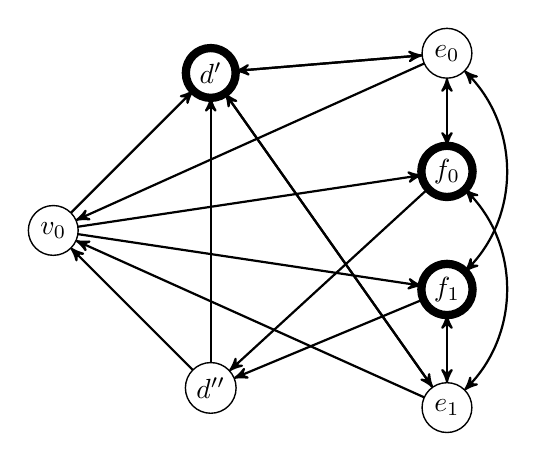
\begin{tikzpicture}[>=stealth']
\SetVertexMath
\Vertex[x=0,y=0.0]{v_0}
\Vertex[x=2,y=-2]{d''}
\Vertex[x=5,y=2.25]{e_0}
\Vertex[x=5,y=-2.25]{e_1}

\renewcommand*{\VertexLineWidth}{3pt}
\Vertex[x=2,y=2]{d'}
\Vertex[x=5,y=0.75]{f_0}
\Vertex[x=5,y=-0.75]{f_1}
\SetUpEdge[style=->]
\Edge(v_0)(d')
\Edges(d',e_0,d')
\Edges(d',e_1,d')
\Edge(d'')(v_0)
\Edges(f_0,e_0,f_0)
\Edges(f_1,e_1,f_1)
\Edge[style={<->,out=45,in=-45}](e_1)(f_0)
\Edge[style={<->,out=-45,in=45}](e_0)(f_1)
\Edge(v_0)(f_0)
\Edge(v_0)(f_1)
\Edge(f_0)(d'')
\Edge(f_1)(d'')
\Edge(e_0)(v_0)
\Edge(e_1)(v_0)
\Edge(d'')(d')

\end{tikzpicture}


    \caption{Graph for the Rollon-Rolloff problem. Thick vertices (except
    $v_0$) represent nodes from which the vehicle leaves loaded. Thin vertices
    are the ones from which it leaves unloaded.}
    \label{fig:avrp-rr}
  \end{center}
\end{figure}

This can now be modeled as an instance of AVRP. The costs $c_{ij}$ associated
with each arc are further detailed in \citet{Aringhieri04}.  $\delta^+(v)$ is
defined as the out-neighborhood of $v$ and $\delta^-(v)$ as its
in-neighborhood. Without the time constraints, the following formulation is
obtained:

\begin{align}
	\mbox{Minimize} & \quad K_A \sum_{(i, j) \in A} c_{ij} x_{ij} +
				K_B \sum_{j \in \delta^-(v_0)} x_{v_0j}
	\\
	\mbox{subject to} & \notag{}
	\\
	\forall_{i \in F \cup E} & \quad \sum_{j \in \delta^+(i)} x_{ij} = 1
	\label{avrp-rr:indegree}
	\\
	\forall_{i \in V} & \quad \sum_{j \in \delta^+(i)} x_{ij} = \sum_{j \in \delta^-(i)} x_{ji}
	\label{avrp-rr:in-out}
	\\
	& \quad \sum_{j \in V} x_{0j} \leq U \label{avrp-rr:upper-k} \\
	& \quad \sum_{j \in V} x_{0j} \geq L \label{avrp-rr:lower-k} \\
	\forall_{i \in D^\prime \cup D^{\prime\prime}} & \quad \sum_{j \in \delta^+(i)} x_{ij} \leq 1 \\
	\forall_{i, j \in V} & \quad x_{ij} \in \{0, 1\}
\end{align}

Although the graph is not complete, the missing arcs can be added with a
arbitrarily large value. If the restrictions described in
section~\ref{section:problem} need to be enforced, it is enough to limit the arcs on
the specified request. Say that the container from $f_0$ must return to $e_0$.
Removing the ingoing edges to $e_0$ and the outgoing edges from $f_0$ (except
the one that connects $f_0$ to $e_0$) is enough to ensure this constraint.




\subsubsection{Solving approaches}
\label{section:rrvrp-approaches}

Solving RRVRP instances, as modeled in the previous section, can be done using
the algorithms described in section~\ref{section:vrp-approaches}.


\section{Chapter summary}

This chapter presented some background information regarding waste collection
problems. It followed by giving a general overview of the modelation of route
optimization problems.

Finally, section~\ref{section:waste-collection-scenarios} presents the
application of route optimization models to waste collection vehicle route
optimization problem. Three different scenarios were introduced.

In the \textit{residential} scenario, there are several approaches applied to
the directed CARP. Although some have been adapted to the undirected variant,
further study could be made regarding the remaining algorithms --- namely, the
usage of metaheuristics.

The \textit{Rollon-rolloff} scenario was formulated as a AVRP instance. Although
the authors provided preliminary computational results using an heuristic, further
computations could be made, comparing several other heuristics, metaheuristics and
exact methods.

The \textit{commercial} scenario is modeled as a \textit{Capacitated Vehicle
Routing Problem}. This model is used whenever the density of waste containers
per street is low.

The next chapter, chapter~\ref{chap:problem}, uses the definitions introduced in
these sections to explicitly state the goals of this study.

\chapter{Specification}
\label{chap:specification}

\section*{}



\chapter{Implementation}
\label{chap:implementation}

\section*{}
Here be dragons.

\section{Map generation and retrieval}
\label{section:map-generation}

To simulate the waste generation and collection, there is the need to provide a
topological city map. This topological map must be represented as a directed
weighted graph, so that routing algorithms may be applied. Being that a city is
usually a sparse graph, I opted for a adjacency list representation. To obtain
the maps, two different approaches were implemented.

First, I implemented the generation of random cities based on the official
RoboCup Rescue simulator. This procedure is detailed in
Section~\ref{section:roborescue}.

I also developed a more realistic approach, described in
Section~\ref{section:osm}  --- a procedure which allows the importation of city
maps from OpenStreetMap.org.




\subsection{RoboCup Rescue Random City Generation}
\label{section:roborescue}

RoboCup Rescue is a competition in which the participants must build agents to
control robot rescue teams, aiming to save the maximum number of people in a
city, after a catastrophe, such as an earthquake. This competition also
requires a city graph, so that the rescue vehicles can navigate through it.
The official simulator contains a procedure for the generation of random
cities, which is described by Teutenberg\citep{Teutenberg03}. Next, it is
presented a short description of this procedure:

\begin{enumerate}
	\item generate a uniformly distributed rectangular grid
	\item randomly shift each intersection in both axis
	\item remove random roads
	\item subdivide overlapping roads, by creating new intersections
	\item weight the roads, according to their usage based on a random set of paths
	\item smooth main roads
\end{enumerate}

As noted in the User's guide, the fourth step implementation is not correctly
implemented. This, along with other references to implementation problems, led
us to write the generator from scratch.

To implement the road intersection removal, there is a widely known algorithm
by Bentley and Ottman\cite{bentley-ottman} whose running time --- $O((n + k)
log~n)$, with $n$ being the number of roads and $k$ the number of overlaps ---
is significantly lower than the naive technique of checking each pair of
segments, which runs in $O(n^2)$.

\begin{figure}[h]
\centering
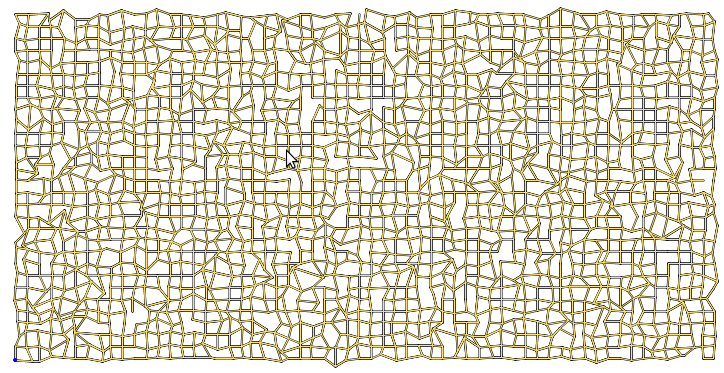
\includegraphics[width=0.75\textwidth]{random_map.png}
\caption{A random city map, generated using RoboCup Rescue official generator}
\label{fig:random_map}
\end{figure}

The maps obtained using this method, as seen in figure~\ref{fig:random_map},
have a grid-like topology. This trait gives them an unrealistic look, which may
be seen as a disadvantage. Regardless of this, maps obtained using this method
may be useful. By tweaking the procedure's parameters, one can obtain city maps
very different from each other, such as the one in
figure~\ref{fig:chaotic_map}. This may be used an easy way to generate
scenarios in which different routing algorithms can be applied, benchmarked and
compared.

\begin{figure}[h]
\centering
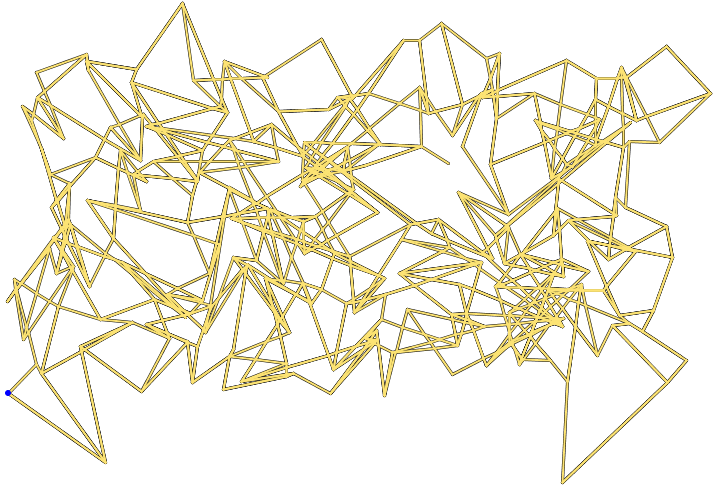
\includegraphics[width=0.75\textwidth]{chaotic_map.png}
\caption{By tweaking parameters of the RoboCup Rescue procedure, different maps can be obtained}
\label{fig:chaotic_map}
\end{figure}




\subsection{\osm{} Data Retrieval}
\label{section:osm}

Random maps may be used for simulation and benchmarking purposes, but there's
also the need to obtain real city maps. In order to obtain this information, an
application that imports maps from \osm{} --- whose data are free for use ---
was developed.  In figure~\ref{fig:porto} we present an example of a city
imported from \osm{}.

\begin{figure}[th]
  \begin{center}
    \leavevmode
    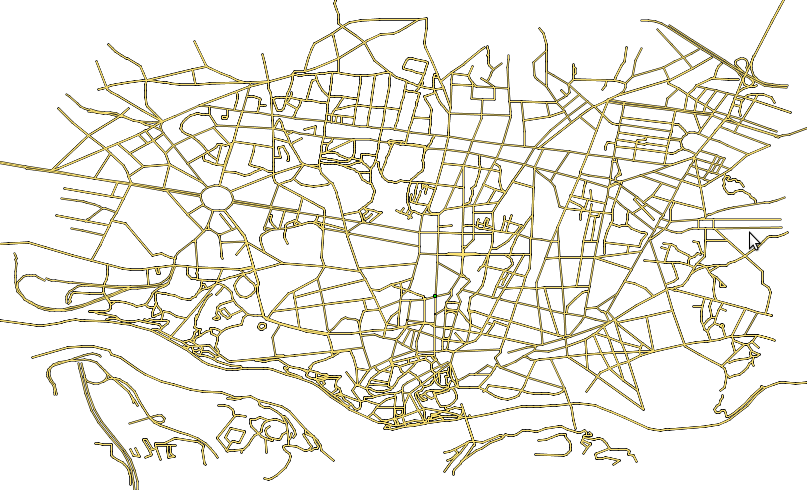
\includegraphics[width=0.75\textwidth]{porto}
    \caption{The city of Porto, Portugal, retrieved from \osm{} and loaded onto the current framework viewer.}
    \label{fig:porto}
  \end{center}
\end{figure}





\subsection{Stochastic waste generation parameters}
\label{section:parameters}

Each containers' fill rate varies according to several parameters, such as the
population density of the surrounding blocks, the socioeconomic level, the time
of the year and the area type --- residential, commercial or industrial, for
example. These topics were studied by Gómez et al, regarding the city of
Chihuahua, México in 2006\citep{Gomez20092018,Gomez20082465}.

As the correlation between these parameters and the waste generation rate is
not yet established (due to the lack of a fill status monitoring system), they
must be estimated. This can be done using the population density of the city
and data on kilograms per capita per day.






%%\chapter{Work Plan}\label{chap:work}
\chapter{Approach}
\label{chap:approach}

\section*{}

This project is structured in a modular way; this chapter enumerates and
describes each one of the modules, defining what is required and produced in
each step. Three main modules were designed, and the general workflow is
described in section~\ref{section:workflow}, with the main modules being
explained in the following sections.

Then, all the data interchange formats are formally specified.



\section{Workflow}
\label{section:workflow}




The framework development has already been started. This chapter details the
work done so far, along with 
The optimisation framework is currently divided into three main modules.

The first module --- described in section~\ref{section:map-generation} ---
regards the generation or retrieval of a problem set. This involves obtaining a
city map, determining containers' locations and associating them with the
current fill status. 

The second module refers to the actual route optimisation, which is made using
a stochastic route simulation to introduce randomness --- representing
fluctuations in the vehicles' speed, for example. Details referring this module
are given in section~\ref{section:simulation}.

There is the need for an analysis and visualization module that takes the
output from the optimisation module and displays it in a human-viewable
fashion, along with several statistics. This module is presented in
section~\ref{section:visualisation}.

\section{Map generation and retrieval}
\label{section:map-generation}

To simulate the waste generation and collection, there is the need to provide a
topological city map. This topological map must be represented as a directed
weighted graph, so that routing algorithms may be applied. Being that a city is
usually a sparse graph, I opted for a adjacency list representation. To obtain
the maps, two different approaches were implemented.

First, I implemented the generation of random cities based on the official
RoboCup Rescue simulator. This procedure is detailed in
Section~\ref{section:roborescue}.

I also developed a more realistic approach, described in
Section~\ref{section:osm}  --- a procedure which allows the importation of city
maps from OpenStreetMap.org.

\subsection{RoboCup Rescue Random City Generation}
\label{section:roborescue}

RoboCup Rescue is a competition in which the participants must build agents to
control robot rescue teams, aiming to save the maximum number of people in a
city, after a catastrophe, such as an earthquake. This competition also
requires a city graph, so that the rescue vehicles can navigate through it.
The official simulator contains a procedure for the generation of random
cities, which is described by Teutenberg\citep{Teutenberg03}. Next, it is
presented a short description of this procedure:

\begin{enumerate}
	\item generate a uniformly distributed rectangular grid
	\item randomly shift each intersection in both axis
	\item remove random roads
	\item subdivide overlapping roads, by creating new intersections
	\item weight the roads, according to their usage based on a random set of paths
	\item smooth main roads
\end{enumerate}

As noted in the User's guide, the fourth step implementation is not correctly
implemented. This, along with other references to implementation problems, led
us to write the generator from scratch.

To implement the road intersection removal, there is a widely known algorithm
by Bentley and Ottman\cite{bentley-ottman} whose running time --- $O((n + k)
log~n)$, with $n$ being the number of roads and $k$ the number of overlaps ---
is significantly lower than the naive technique of checking each pair of
segments, which runs in $O(n^2)$.

\begin{figure}[h]
\centering
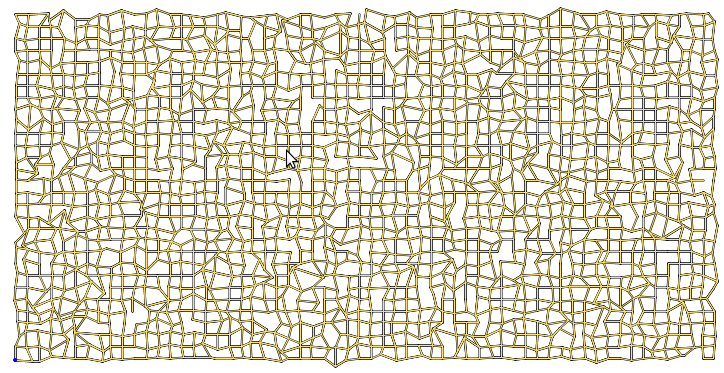
\includegraphics[width=0.75\textwidth]{random_map.png}
\caption{A random city map, generated using RoboCup Rescue official generator}
\label{fig:random_map}
\end{figure}

The maps obtained using this method, as seen in figure~\ref{fig:random_map},
have a grid-like topology. This trait gives them an unrealistic look, which may
be seen as a disadvantage. Regardless of this, maps obtained using this method
may be useful. By tweaking the procedure's parameters, one can obtain city maps
very different from each other, such as the one in
figure~\ref{fig:chaotic_map}. This may be used an easy way to generate
scenarios in which different routing algorithms can be applied, benchmarked and
compared.

\begin{figure}[h]
\centering
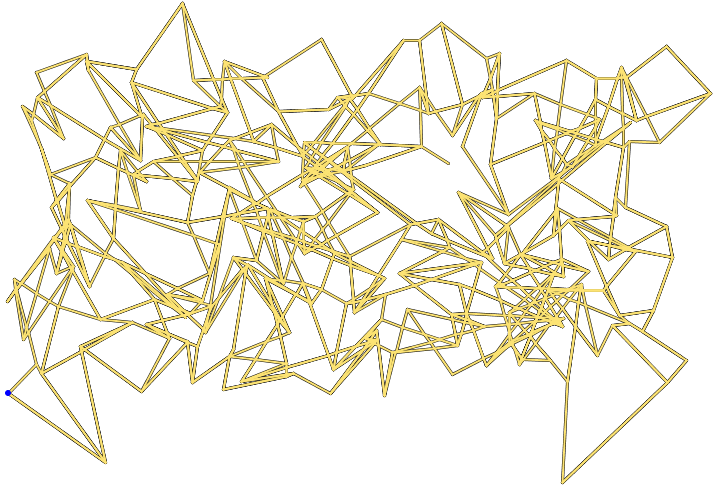
\includegraphics[width=0.75\textwidth]{chaotic_map.png}
\caption{By tweaking parameters of the RoboCup Rescue procedure, different maps can be obtained}
\label{fig:chaotic_map}
\end{figure}



\subsection{\osm{} Data Retrieval}
\label{section:osm}

Random maps may be used for simulation and benchmarking purposes, but there's
also the need to obtain real city maps. In order to obtain this information, an
application that imports maps from \osm{} --- whose data are free for use ---
was developed.  In figure~\ref{fig:porto} we present an example of a city
imported from \osm{}.

\begin{figure}[th]
  \begin{center}
    \leavevmode
    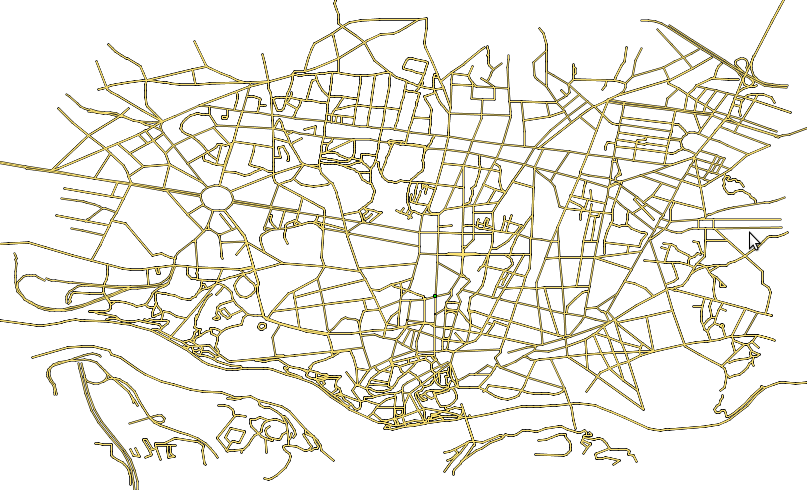
\includegraphics[width=0.75\textwidth]{porto}
    \caption{The city of Porto, Portugal, retrieved from \osm{} and loaded onto the current framework viewer.}
    \label{fig:porto}
  \end{center}
\end{figure}



\subsection{Stochastic waste generation parameters}
\label{section:parameters}

Each containers' fill rate varies according to several parameters, such as the
population density of the surrounding blocks, the socioeconomic level, the time
of the year and the area type --- residential, commercial or industrial, for
example. These topics were studied by Gómez et al, regarding the city of
Chihuahua, México in 2006\citep{Gomez20092018,Gomez20082465}.

As the correlation between these parameters and the waste generation rate is
not yet established (due to the lack of a fill status monitoring system), they
must be estimated. This can be done using the population density of the city
and data on kilograms per capita per day.








\section{Route Optimisation and Evaluation}
\label{section:simulation}

Before applying the optimisation techniques to the real world scenario, several
tests need to be done, comparing several algorithms. These tests will be
executed on a simulator, whose behaviour is defined in this section.

The simulation process starts by loading the problem set and connecting ---
through a network socket -- to the optimiser, which implements the optimisation
algorithm. The choice of using a network socket was made to keep these two
components completely independent, in order not to hinder the development of
new optimisation techniques.

The communication protocol between these two components is simple. The
simulator starts by sending the city map to the optimiser. Afterwards, for each
day of simulation, the simulator sends the containers' state to the optimiser
and receives the routes to apply, at the end of the day. This is depicted in
figure~\ref{fig:protocol}, with steps 2 and 3 being executed once for each day.

\begin{figure}[th]
\centering
% Graphic for TeX using PGF
% Title: /home/hugopeixoto/Diagram1.dia
% Creator: Dia v0.97
% CreationDate: Fri Jan 22 10:26:00 2010
% For: hugopeixoto
% \usepackage{tikz}
% The following commands are not supported in PSTricks at present
% We define them conditionally, so when they are implemented,
% this pgf file will use them.
\ifx\du\undefined
  \newlength{\du}
\fi
\setlength{\du}{15\unitlength}
\begin{tikzpicture}
\pgftransformxscale{1.000000}
\pgftransformyscale{-1.000000}
\definecolor{dialinecolor}{rgb}{0.000000, 0.000000, 0.000000}
\pgfsetstrokecolor{dialinecolor}
\definecolor{dialinecolor}{rgb}{1.000000, 1.000000, 1.000000}
\pgfsetfillcolor{dialinecolor}
\pgfsetlinewidth{0.100000\du}
\pgfsetdash{}{0pt}
\pgfsetdash{}{0pt}
\pgfsetbuttcap
{
\definecolor{dialinecolor}{rgb}{0.000000, 0.000000, 0.000000}
\pgfsetfillcolor{dialinecolor}
% was here!!!
\pgfsetarrowsend{stealth}
\definecolor{dialinecolor}{rgb}{0.000000, 0.000000, 0.000000}
\pgfsetstrokecolor{dialinecolor}
\draw (36.493750\du,13.000000\du)--(46.360625\du,13.020000\du);
}
\definecolor{dialinecolor}{rgb}{1.000000, 1.000000, 1.000000}
\pgfsetfillcolor{dialinecolor}
\fill (32.000000\du,12.000000\du)--(32.000000\du,17.000000\du)--(36.493750\du,17.000000\du)--(36.493750\du,12.000000\du)--cycle;
\pgfsetlinewidth{0.100000\du}
\pgfsetdash{}{0pt}
\pgfsetdash{}{0pt}
\pgfsetmiterjoin
\definecolor{dialinecolor}{rgb}{0.000000, 0.000000, 0.000000}
\pgfsetstrokecolor{dialinecolor}
\draw (32.000000\du,12.000000\du)--(32.000000\du,17.000000\du)--(36.493750\du,17.000000\du)--(36.493750\du,12.000000\du)--cycle;
% setfont left to latex
\definecolor{dialinecolor}{rgb}{0.000000, 0.000000, 0.000000}
\pgfsetstrokecolor{dialinecolor}
\node at (34.246875\du,14.695000\du){Simulator};
\definecolor{dialinecolor}{rgb}{1.000000, 1.000000, 1.000000}
\pgfsetfillcolor{dialinecolor}
\fill (46.360625\du,12.020000\du)--(46.360625\du,17.000000\du)--(50.970625\du,17.000000\du)--(50.970625\du,12.020000\du)--cycle;
\pgfsetlinewidth{0.100000\du}
\pgfsetdash{}{0pt}
\pgfsetdash{}{0pt}
\pgfsetmiterjoin
\definecolor{dialinecolor}{rgb}{0.000000, 0.000000, 0.000000}
\pgfsetstrokecolor{dialinecolor}
\draw (46.360625\du,12.020000\du)--(46.360625\du,17.000000\du)--(50.970625\du,17.000000\du)--(50.970625\du,12.020000\du)--cycle;
% setfont left to latex
\definecolor{dialinecolor}{rgb}{0.000000, 0.000000, 0.000000}
\pgfsetstrokecolor{dialinecolor}
\node at (48.665625\du,14.705000\du){Optimizer};
% setfont left to latex
\definecolor{dialinecolor}{rgb}{0.000000, 0.000000, 0.000000}
\pgfsetstrokecolor{dialinecolor}
\node at (41.427187\du,12.457500\du){1. send\_map};
\pgfsetlinewidth{0.100000\du}
\pgfsetdash{}{0pt}
\pgfsetdash{}{0pt}
\pgfsetbuttcap
{
\definecolor{dialinecolor}{rgb}{0.000000, 0.000000, 0.000000}
\pgfsetfillcolor{dialinecolor}
% was here!!!
\pgfsetarrowsend{stealth}
\definecolor{dialinecolor}{rgb}{0.000000, 0.000000, 0.000000}
\pgfsetstrokecolor{dialinecolor}
\draw (36.493750\du,14.500000\du)--(46.360625\du,14.510000\du);
}
\pgfsetlinewidth{0.100000\du}
\pgfsetdash{}{0pt}
\pgfsetdash{}{0pt}
\pgfsetbuttcap
{
\definecolor{dialinecolor}{rgb}{0.000000, 0.000000, 0.000000}
\pgfsetfillcolor{dialinecolor}
% was here!!!
\pgfsetarrowsend{stealth}
\definecolor{dialinecolor}{rgb}{0.000000, 0.000000, 0.000000}
\pgfsetstrokecolor{dialinecolor}
\draw (46.360625\du,16.000000\du)--(36.493750\du,16.000000\du);
}
% setfont left to latex
\definecolor{dialinecolor}{rgb}{0.000000, 0.000000, 0.000000}
\pgfsetstrokecolor{dialinecolor}
\node at (41.427187\du,15.447500\du){3. send routes};
% setfont left to latex
\definecolor{dialinecolor}{rgb}{0.000000, 0.000000, 0.000000}
\pgfsetstrokecolor{dialinecolor}
\node at (41.427187\du,13.952500\du){2. send state};
\end{tikzpicture}

\caption{Communication protocol during the simulation}
\label{fig:protocol}
\end{figure}

Routes received from the optimiser are composed by a set of intersection
points the vehicle must follow. For each road segment, the simulator
determines the vehicle speed, following a normal distribution --- which will
be configurable. This provides the simulation with some reality and
nondeterminism. 

This will cause situations like the ones described at the end of
Section~\ref{section:problem}, in which a vehicle has to wait for another one
to finish a given task.

The time it takes for a vehicle to empty or load a container is also
determined by a normal distribution.

Each event, timestamp and vehicle speed is registered in a log file, for
further inspection and evaluation. The routes are also registered, as well as
the average distance per day.






\section{Visualisation}
\label{section:visualisation}

After obtaining the log file from the simulation module, one can check the
collection process in the viewer, step by step. For example, it is possible
to verify, in the replacement variation, when a vehicle is idling, waiting
for another one. A screenshot of the current viewer's prototype is available
in figure~\ref{fig:simulation}.

\begin{figure}[h]
\centering
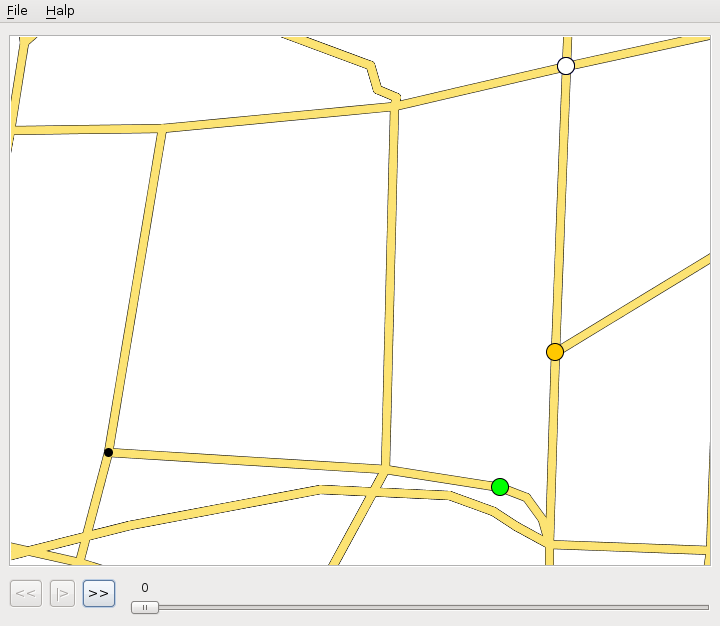
\includegraphics[width=0.75\textwidth]{simulation.png}
\caption{Screenshot of the viewer, showing a container (black, smaller circle)
and three vehicles in different states. Green: moving, white: finished, orange:
collecting the waste.}
\label{fig:simulation}
\end{figure}

This viewer can easily be extended to read and display extra information from
the log file, such as other performance metrics. Currently, it also supports
the functionality of loading a stand alone city map, so that inconsistencies
may be detected before running the optimisation procedures.

The next steps include creating a front-end to place the containers' around
the city and to display detailed information regarding the optimisation
process.



%\chapter{Work Plan}\label{chap:work}

\section*{}

This chapter defines roughly the work plan for the next five months, in which
the research will be completed. Section~\ref{section:tasks} starts by defining
a major set of tasks, subsequently dividing each one into subtasks. It also
provides an estimated time for each one.

Then, in section~\ref{section:calendarisation}, these tasks are scheduled along
the next five months.

\section{Tasks}
\label{section:tasks}

In order to successfully employ an optimisation solution, I will develop a
simple framework for the evaluation of optimisation algorithms. This work has
already been started, but still needs some refinement. Once this is done, I
shall work on implement the optimisation techniques and develop the
architecture for communicating with the monitoring central system. I will also
compare these algorithms and provide benchmarks. As soon as these tasks are
done, I will focus on writing the thesis.

Next, I present a list with these tasks, their detailed description and an
estimated time. Figure~\ref{fig:gantt} shows a Gantt diagram with these tasks'
scheduling.

\begin{description}
\item[Framework] \hfill \\
Development of a framework for the evaluation and benchmark of optimisation
techniques. This involves finishing and polishing all modules described in
chapter~\ref{chap:approach}. This can be divided into the following subtasks:

\begin{itemize}
	\item Development of a tool that allows the editing of a city's containers and their fill rates;
	\item Implementation of the optimisation visualisation tool.
\end{itemize}

Estimated time: 4 weeks.

\item[Architecture] \hfill \\
Definition of an architecture for the communication between the optimisation
framework and the monitoring system.

\begin{itemize}
	\item Study of the current state on the fill status monitoring system;
	\item Design of a simple database to store information;
	\item Specify protocols for accessing and updating data.
\end{itemize}


Estimated time: 4 weeks.

\item[Optimisation] \hfill \\
Implementation and further study of different optimisation algorithms. This
requires the development of several heuristics, metaheuristics and exact methods
for both the \textit{commercial} and the \textit{rollon-rolloff} scenarios.

\begin{itemize}
	\item \textit{commercial} exact methods;
	\item \textit{commercial} heuristics;
	\item \textit{commercial} metaheuristics;
	\item adapt the \textit{commercial} approaches to the \textit{rollon-rolloff} scenario.
\end{itemize}

Estimated time: 8 weeks.

\item[Comparison] \hfill \\
Gathering of data to provide a solid comparison and benchmark of the
implemented algorithms. This task will also require parameter tuning and
sensibility analysis.


Estimated time: 4 weeks.

\item[Thesis writing] \hfill \\
Thesis writing, including a detailed documentation of the optimisation
techniques and their performance. Estimated time: 4 weeks.

\end{description}


\newpage
\section{Calendarisation}
\label{section:calendarisation}

Here, I present the calendarisation of the previously specified tasks.  Tasks
\textit{Framework} and \textit{Architecture} overlap because the framework will
eventually need to receive data from the fill status monitoring system.  Tasks
\textit{Architecture} and \textit{Optimisation} can be done interchangeably, as
they are independent. Finally, tasks \textit{Optimisation} and
\textit{Comparison} will slightly overlap because as the comparison between
techniques is done, further insight on their properties may provide clues to
their improvement.

\vspace{2cm}

\begin{figure}[th]
  \begin{center}
    \leavevmode

    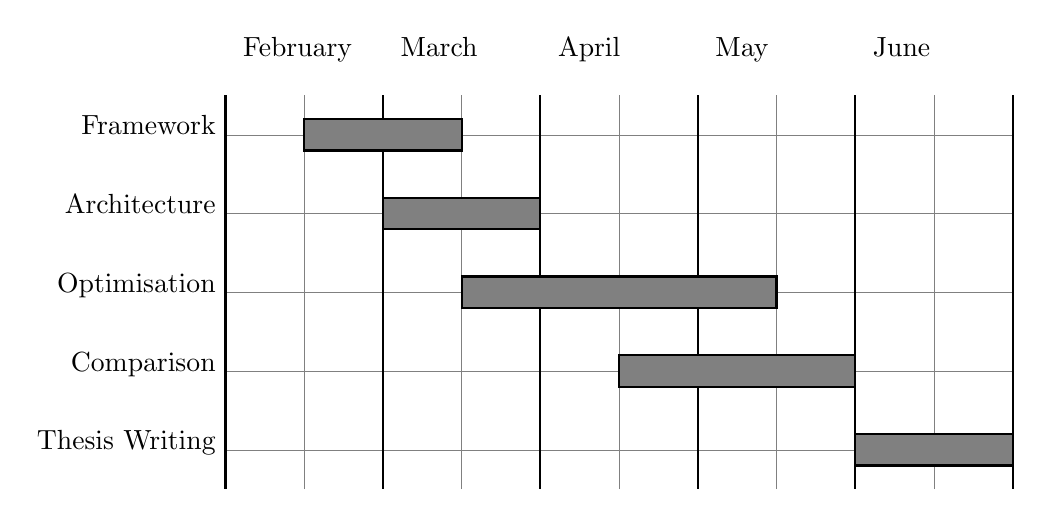
\begin{tikzpicture}[y=-1cm]
      \draw[help lines] (0,5.5) grid (10,0.5);
      \draw[thick] (0,0.5) -- (0,5.5);
      \draw[thick] (2,0.5) -- (2,5.5);
      \draw[thick] (4,0.5) -- (4,5.5);
      \draw[thick] (6,0.5) -- (6,5.5);
      \draw[thick] (8,0.5) -- (8,5.5);
      \draw[thick] (10,0.5) -- (10,5.5);
      
      \node at (0.1,0.0) [anchor=base west] {February};
      \node at (2.1,0.0) [anchor=base west] {March};
      \node at (4.1,0.0) [anchor=base west] {April};
      \node at (6.1,0.0) [anchor=base west] {May};
      \node at (8.1,0.0) [anchor=base west] {June};
      
      \ganttline{1}{Framework}{15}{45}
      \ganttline{2}{Architecture}{30}{60}
      \ganttline{3}{Optimisation}{45}{105}
      \ganttline{4}{Comparison}{75}{120}
      \ganttline{5}{Thesis Writing}{120}{150}
    \end{tikzpicture}

    \caption{Diagram containing the calendarisation of the tasks.}
    \label{fig:gantt}
  \end{center}
\end{figure}



%%----------------------------------------
%% Final materials
%%----------------------------------------

%\bibliographystyle{unsrt}
\begin{singlespace}
  %% Bibliography
  %% Comment the next command if BibTeX file not used, 
  %% bibliography is in ``myrefs.bib''
  \PrintBib{myrefs}

  %% Index
  %% Uncomment next command if index is required,
  %% don't forget to run ``makeindex mieic'' command
  %\PrintIndex

  %% Comment next 2 commands if numbered appendixes not used
  %\appendix
  %\include{appendix1}
\end{singlespace}

\end{document}
